% ======================================================================
% SECTION 05: STORYTELLING SUMMARY — ANALYTICAL AGGREGATIONS & NARRATIVE
% ======================================================================
\section{Storytelling Summary --- Analytical Aggregations and Narrative}

\subsection{Dashboard Narrative and Functional User Alignment}
In Workshop~\#1, we defined our primary functional user as a \textbf{Civil Protection \& Seismic Risk Analyst} responsible for monitoring global and regional seismic activity, distinguishing routine background tectonic release from anomalous earthquake swarms or major destructive ruptures, and assessing cross-agency reporting reliability.

A raw table of thousands of earthquakes overwhelms operational decision-making because micro-earthquakes ($M < 3.0$) dominate event counts ($54.07\%$ of records) while contributing negligible tectonic energy, whereas rare $M \ge 5.5$ ruptures ($2.39\%$ of records) release over $99\%$ of radiated seismic energy. Our storytelling narrative guides the analyst from macro-level hazard state to granular regional and catalog insights:
\begin{enumerate}
    \item \emph{``Is global seismic activity currently normal or anomalous?''} Answered by the daily \textbf{Seismic Activity Anomaly Index (SAAI)} trend, which combines frequency Z-scores ($40\%$ weight) and logarithmic energy Z-scores ($60\%$ weight).
    \item \emph{``How is seismic activity distributed across severity tiers and focal depths?''} Answered by the Gutenberg-Richter severity class distribution and the Shallow/Intermediate/Deep focal depth regime breakdown (since shallow $<70\,\text{km}$ ruptures account for $88.60\%$ of events and pose the highest Peak Ground Acceleration hazard).
    \item \emph{``Which tectonic regions are experiencing peak activity right now, and how do international agencies compare?''} Answered by the Top 15 Active Seismic Regions ranking and the multi-source catalog comparison across USGS, EMSC, and GDACS.
\end{enumerate}

\subsection{Storytelling Aggregations and User Story Mapping}
All five analytical aggregations are computed in PySpark and persisted in \texttt{datalake\_gold/storytelling\_YYYYMMDD\_HHMMSS.parquet} ($84$ rows $\times$ $14$ columns), partitioned logically by \texttt{aggregation\_type}. Table~\ref{tab:storytelling_mapping} maps each aggregation to its Workshop~\#1 User Story and target Workshop~\#4 Plotly Dash component.

\begin{table*}[!t]
\centering
\caption{Mapping of Gold Layer Storytelling Aggregations to Workshop \#1 User Stories and Planned Dashboard Components}
\label{tab:storytelling_mapping}
\begin{tabularx}{\textwidth}{llXXX}
\toprule
\textbf{\texttt{aggregation\_type}} & \textbf{User Story} & \textbf{PySpark / Spark SQL Computation Logic} & \textbf{Key Empirical Insight in Gold Parquet} & \textbf{Planned Workshop \#4 Chart} \\
\midrule
\texttt{severity\_distribution} (5 rows) & US-01 (Severity Monitoring) & Spark SQL grouping over 5 Gutenberg-Richter classes: Micro/Minor ($<3.0$), Light ($3.0\text{--}4.4$), Moderate ($4.5\text{--}5.4$), Strong ($5.5\text{--}6.4$), Major ($\ge 6.5$). & Micro/Minor accounts for $54.07\%$ of count ($mean\ M=1.61$), Moderate for $35.39\%$ ($mean\ M=4.78$), and Strong/Major for $2.39\%$ (up to $M=6.80$). & Severity Distribution Bar / Donut Chart \\
\texttt{temporal\_trend\_saai} (47 rows) & US-02 \& US-04 (Anomaly Detection) & Daily aggregation of event frequency $N_t$, cumulative radiated energy $\log_{10}(\sum E_t)$, and composite Z-score $\text{SAAI}(t) = 0.4 Z_N + 0.6 Z_E$. & Identifies elevated anomaly window on \texttt{2026-11-05} ($N=260$, $M_{\max}=6.1$, $\log_{10} E = 14.00$, $\text{SAAI}=1.003$ \texttt{ELEVATED}). & Dual-Axis SAAI \& Daily Seismic Energy Trend Line Chart \\
\texttt{top\_regions\_keywords} (15 rows) & US-03 (Geographic Hotspots) & Regex extraction of clean region names from \texttt{place}, ranked by event count with mean/max magnitude and mean focal depth. & Top micro-seismic swarms in \texttt{The Geysers, CA} ($123$ events) and \texttt{Milford, Utah} ($115$); top moderate/strong clusters in \texttt{Mindanao, Philippines} ($51$ events, $M_{\max}=5.9$). & Top Active Tectonic Regions Horizontal Bar Chart (colored by alert tier) \\
\texttt{source\_comparison} (14 rows) & US-05 (Multi-Agency Trust) & Two-dimensional grouping by \texttt{(source\_id, severity\_tier)} comparing count, share $\%$, and magnitude range across catalogs. & Reveals catalog sensitivity thresholds: \texttt{usgs\_realtime} captures micro-seismicity ($M \ge -0.91$), whereas \texttt{emsc\_fdsn} and \texttt{gdacs\_realtime} focus on $M \ge 4.5$ global hazards. & Multi-Source Agency Comparison Grouped Bar Chart \\
\texttt{depth\_regime\_breakdown} (3 rows) & US-06 (Subduction \& PGA Risk) & Classification into Shallow ($0\text{--}70\,\text{km}$), Intermediate ($70\text{--}300\,\text{km}$), and Deep ($>300\,\text{km}$) regimes. & $88.60\%$ Shallow (mean depth $12.97\,\text{km}$), $9.81\%$ Intermediate ($116.83\,\text{km}$), and $1.59\%$ Deep ($510.66\,\text{km}$, mean $M=4.65$). & Focal Depth Regime Breakdown \& Risk Card \\
\bottomrule
\end{tabularx}
\end{table*}

\begin{figure*}[!t]
\centering
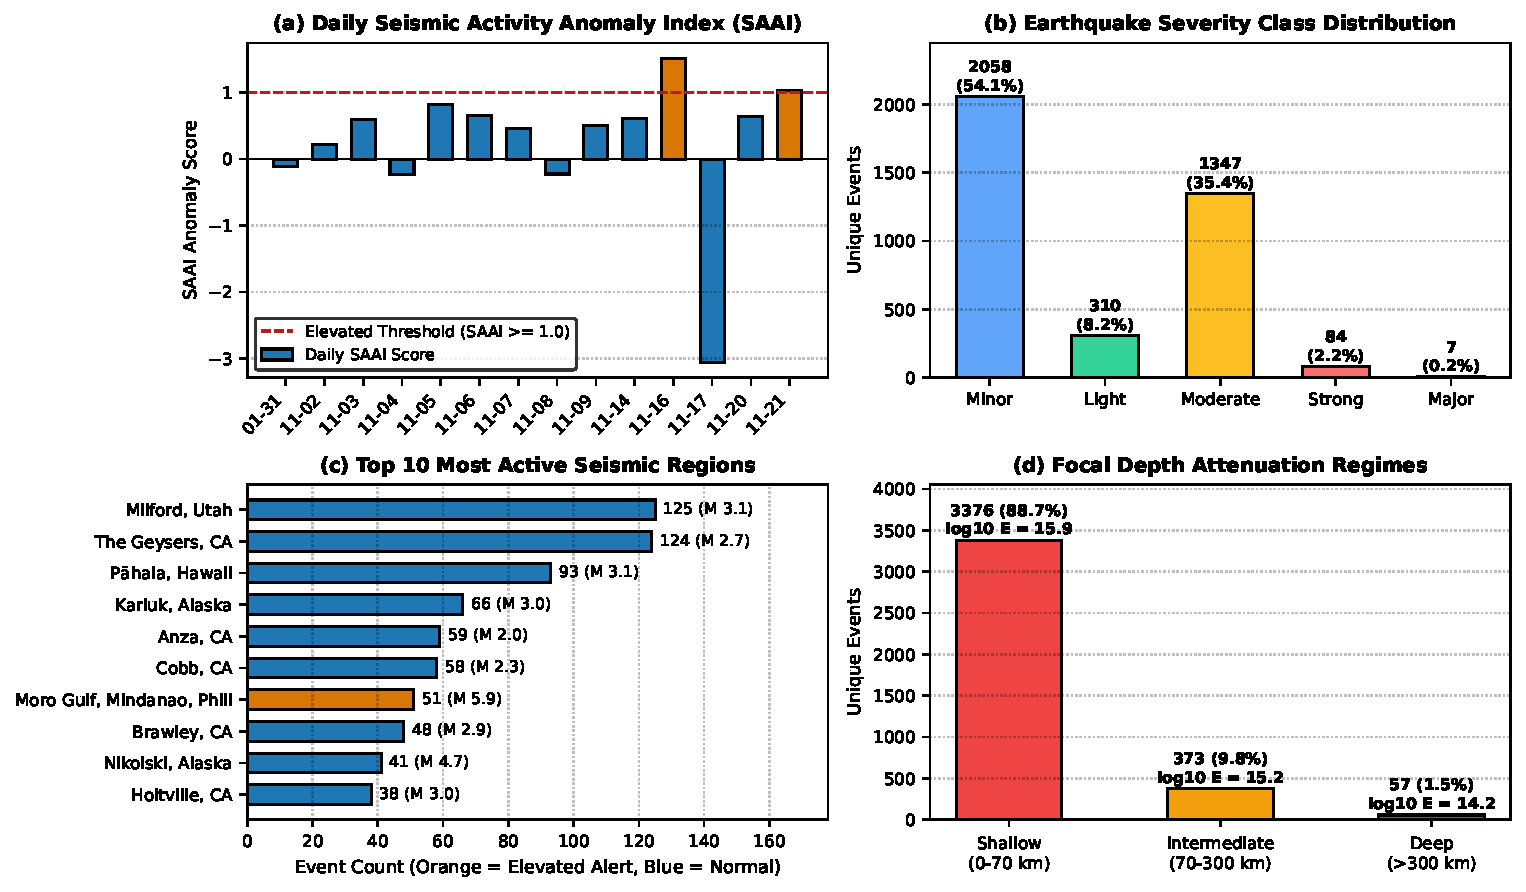
\includegraphics[width=0.96\textwidth]{figures/fig2_gold_storytelling_saai.pdf}
\caption{Gold-layer storytelling analytical visualizations computed from \texttt{datalake\_gold/storytelling\_*.parquet}: Gutenberg-Richter severity class distribution, daily Seismic Activity Anomaly Index (SAAI) time series, top active tectonic regions, and multi-agency catalog comparison.}
\label{fig:gold_storytelling}
\end{figure*}
